% Anexos
% Capítulo de anexos con ejemplos mínimos para incluir capturas y escribir texto explicativo bajo cada imagen.

\appendix

\chapter{Anexos}
\label{ch:anexos}

\section{Figuras: capturas del formulario}
Las siguientes imágenes provienen del formulario recogido en la encuesta. Debajo de cada figura hay una breve descripción.

% 1. edades

\IfFileExists{images/imgAnexos/edades.png}{
	\begin{figure}[H]
		\centering
		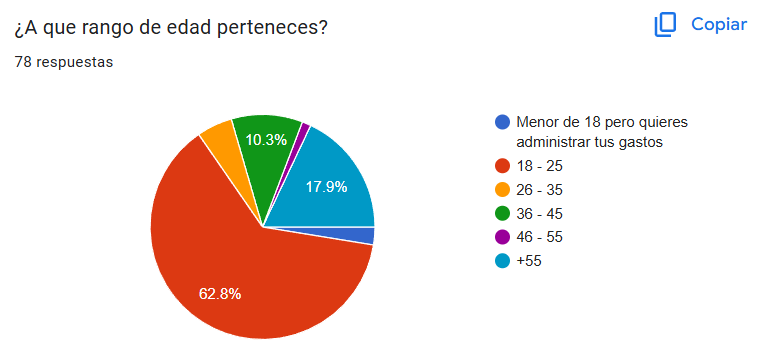
\includegraphics[width=0.8\textwidth]{images/imgAnexos/edades.png}
		\caption{Distribución por rango de edad.}
		\label{fig:edades}
	\end{figure}
	Distribución de edades entre los encuestados; útil para entender la demografía predominante.
}{}

% 2. control

\IfFileExists{images/imgAnexos/control.png}{
	\begin{figure}[H]
		\centering
		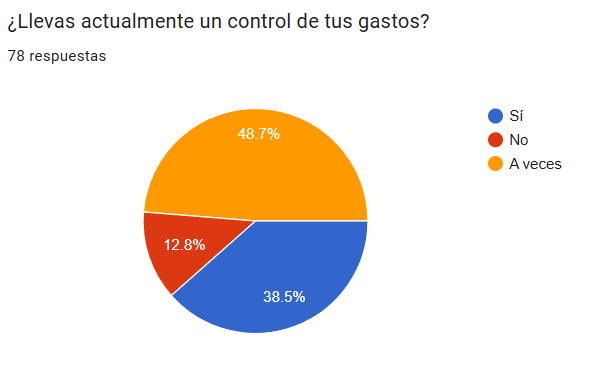
\includegraphics[width=0.8\textwidth]{images/imgAnexos/control.png}
		\caption{Control de gastos actual.}
		\label{fig:control}
	\end{figure}
	Resumen de si los participantes llevan o no un control de sus gastos.
}{}

% 3. esfacilcontrolar

\IfFileExists{images/imgAnexos/esfacilcontrolar.png}{
	\begin{figure}[H]
		\centering
		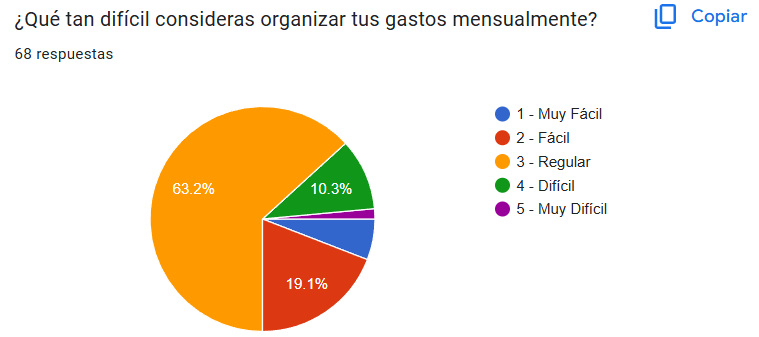
\includegraphics[width=0.8\textwidth]{images/imgAnexos/esfacilcontrolar.png}
		\caption{Percepción sobre la facilidad de organizar gastos.}
		\label{fig:esfacil}
	\end{figure}
	Indica cuánto esfuerzo perciben los usuarios para organizar sus gastos mensuales.
}{}

% 4. porqueahorrar

\IfFileExists{images/imgAnexos/porqueahorrar.png}{
	\begin{figure}[H]
		\centering
		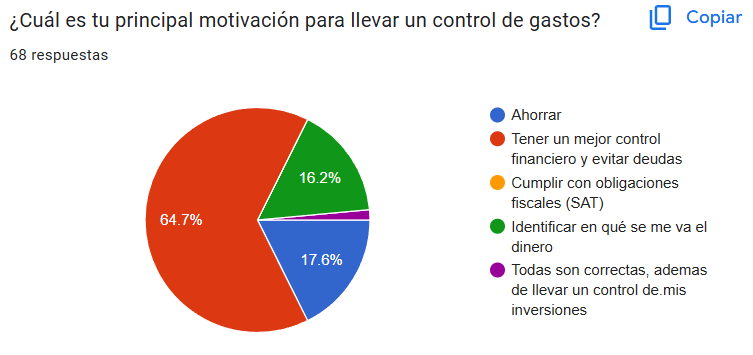
\includegraphics[width=0.8\textwidth]{images/imgAnexos/porqueahorrar.png}
		\caption{Motivaciones para llevar control (por qué ahorrar).}
		\label{fig:porqueahorrar}
	\end{figure}
	Motivos principales que empujan a los usuarios a controlar sus finanzas.
}{}

% 5. has usado alguna aplicacion

\IfFileExists{images/imgAnexos/has usado alguna aplicacion.png}{
	\begin{figure}[H]
		\centering
		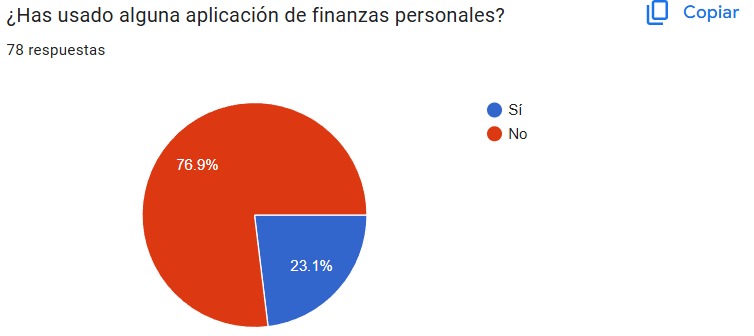
\includegraphics[width=0.8\textwidth]{images/imgAnexos/has usado alguna aplicacion.png}
		\caption{Uso previo de aplicaciones de finanzas personales.}
		\label{fig:hasusado}
	\end{figure}
	Proporción de encuestados que han usado alguna aplicación para finanzas personales.
}{}

% 6. quetegusta

\IfFileExists{images/imgAnexos/quetegusta.png}{
	\begin{figure}[H]
		\centering
		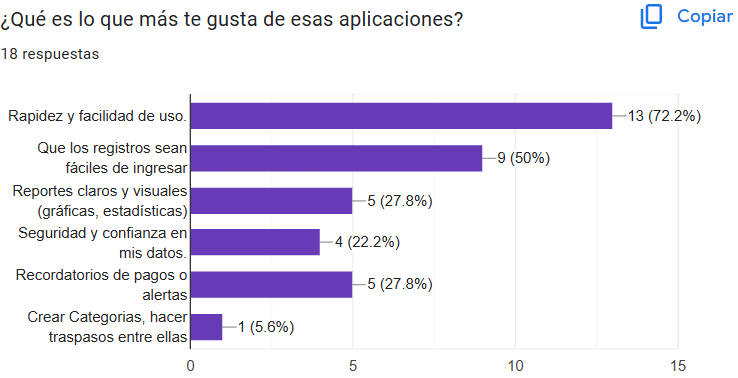
\includegraphics[width=0.8\textwidth]{images/imgAnexos/quetegusta.png}
		\caption{Qué les gusta de las aplicaciones.}
		\label{fig:quetegusta}
	\end{figure}
	Aspectos mejor valorados por los usuarios en las apps de finanzas.
}{}

% 7. problemas de aplicaciones

\IfFileExists{images/imgAnexos/probelmas de aplicaciones.png}{
	\begin{figure}[H]
		\centering
		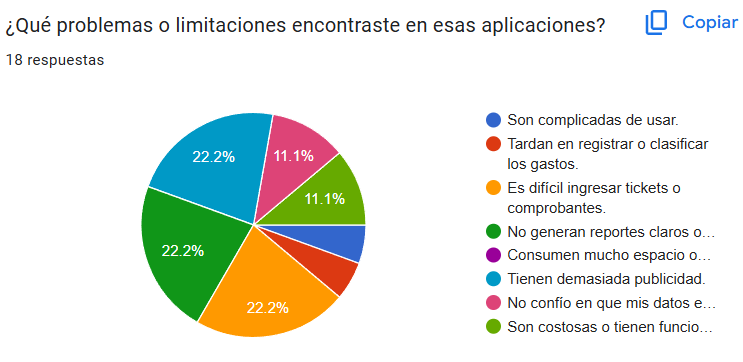
\includegraphics[width=0.8\textwidth]{images/imgAnexos/probelmas de aplicaciones.png}
		\caption{Problemas o limitaciones encontradas en aplicaciones.}
		\label{fig:problemasapps}
	\end{figure}
	Limitaciones que los usuarios han experimentado en apps existentes.
}{}

% 8. guardastickets

\IfFileExists{images/imgAnexos/guardastickets.png}{
	\begin{figure}[H]
		\centering
		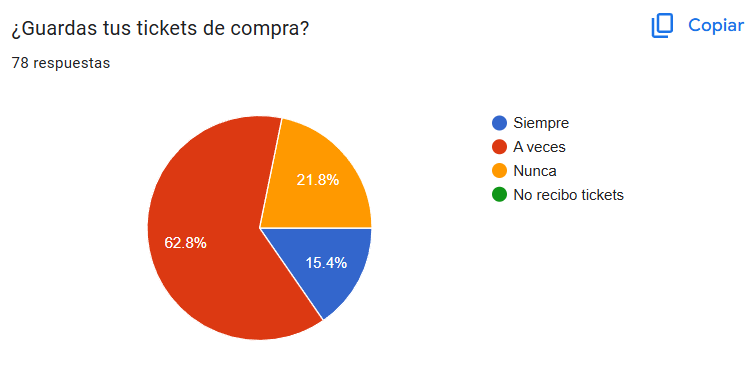
\includegraphics[width=0.8\textwidth]{images/imgAnexos/guardastickets.png}
		\caption{Hábitos de guardar tickets.}
		\label{fig:guardatickets}
	\end{figure}
	Frecuencia con que los encuestados guardan sus comprobantes de compra.
}{}

% 9. tegustariapodertomarfotos

\IfFileExists{images/imgAnexos/tegustariapodertomarfotos.png}{
	\begin{figure}[H]
		\centering
		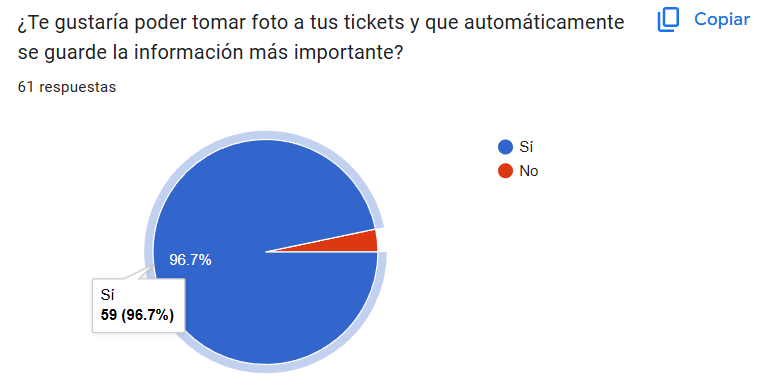
\includegraphics[width=0.8\textwidth]{images/imgAnexos/tegustariapodertomarfotos.png}
		\caption{Interés en tomar fotos de tickets.}
		\label{fig:tomarfotos}
	\end{figure}
	Nivel de interés en usar la función de fotografiar tickets para extraer datos automáticamente.
}{}

% 10. tipos de gastos más comunes

\IfFileExists{images/imgAnexos/tiposdegastomascomunes.png}{
	\begin{figure}[H]
		\centering
		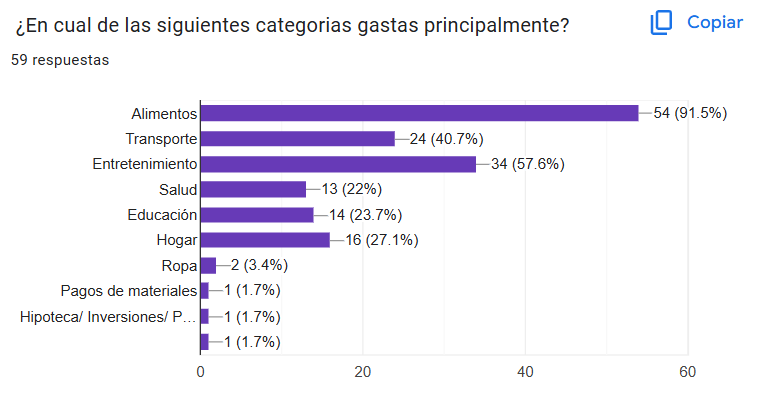
\includegraphics[width=0.8\textwidth]{images/imgAnexos/tiposdegastomascomunes.png}
		\caption{Tipos de gastos más comunes.}
		\label{fig:tiposgastos}
	\end{figure}
	Categorías en las que los encuestados reportan gastar principalmente.
}{}

% 11. tipos de reportes

\IfFileExists{images/imgAnexos/tipos de reportes.png}{
	\begin{figure}[H]
		\centering
		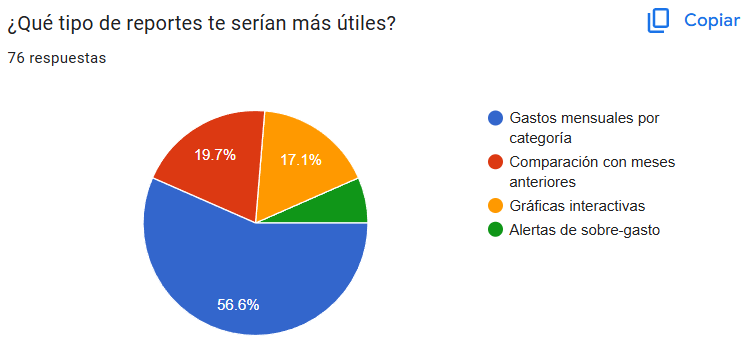
\includegraphics[width=0.8\textwidth]{images/imgAnexos/tipos de reportes.png}
		\caption{Tipos de reportes preferidos.}
		\label{fig:tiposreportes}
	\end{figure}
	Reportes y alertas que los usuarios consideran más útiles.
}{}

% 12. funcionalidades mas utiles

\IfFileExists{images/imgAnexos/funcionalidadmasutil.png}{
	\begin{figure}[H]
		\centering
		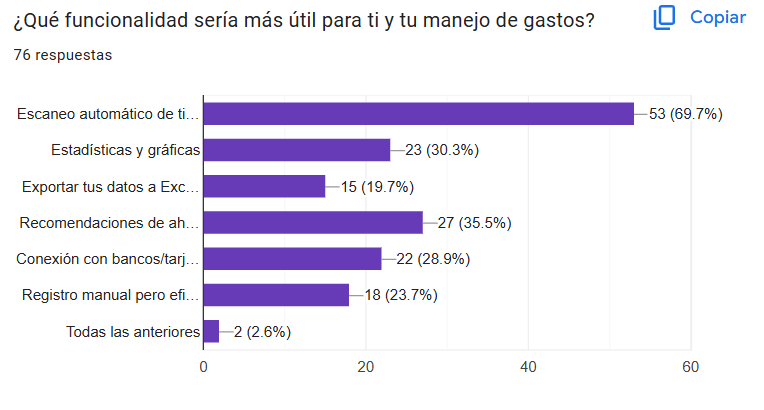
\includegraphics[width=0.8\textwidth]{images/imgAnexos/funcionalidadmasutil.png}
		\caption{Funcionalidades más útiles según los usuarios.}
		\label{fig:funcionalidades}
	\end{figure}
	Funcionalidades priorizadas por los encuestados para el manejo de gastos.
}{}

% ──────────────────────────────────────────────────────────────
\section{Encuesta de pruebas de usabilidad}
\label{sec:anexo-encuesta-pruebas}
% ──────────────────────────────────────────────────────────────

Las siguientes imágenes corresponden a los resultados de la encuesta de usabilidad aplicada a 6 participantes el \textbf{20 de mayo de 2026}, tras interactuar con el sistema FINARA en condiciones reales de uso. Cada gráfica muestra la distribución de respuestas para una de las 11 preguntas del formulario.

\IfFileExists{images/imgAnexosPruebas/facilidad_navegacion.png}{
	\begin{figure}[H]
		\centering
		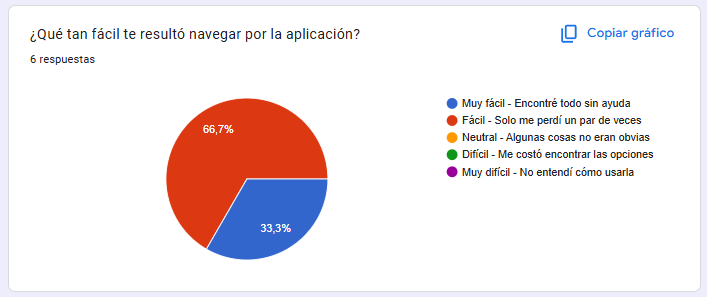
\includegraphics[width=0.8\textwidth]{images/imgAnexosPruebas/facilidad_navegacion.png}
		\caption{Facilidad de navegación en la aplicación.}
		\label{fig:pru-navegacion}
	\end{figure}
	Distribución de respuestas sobre qué tan fácil resultó navegar por la aplicación.
}{}

\IfFileExists{images/imgAnexosPruebas/funcion_escanear_tickets.png}{
	\begin{figure}[H]
		\centering
		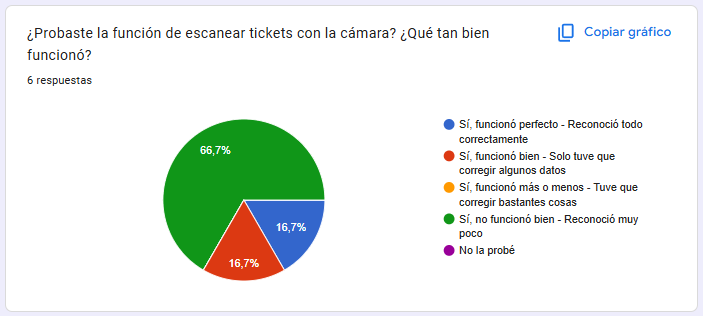
\includegraphics[width=0.8\textwidth]{images/imgAnexosPruebas/funcion_escanear_tickets.png}
		\caption{Desempeño percibido de la función de escaneo de tickets.}
		\label{fig:pru-ocr}
	\end{figure}
	Percepción de los participantes sobre el funcionamiento del módulo OCR.
}{}

\IfFileExists{images/imgAnexosPruebas/diseno_app.png}{
	\begin{figure}[H]
		\centering
		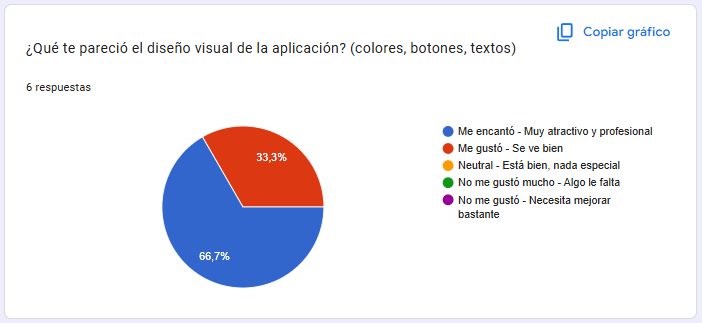
\includegraphics[width=0.8\textwidth]{images/imgAnexosPruebas/diseno_app.png}
		\caption{Valoración del diseño visual de la aplicación.}
		\label{fig:pru-diseno}
	\end{figure}
	Opinión sobre colores, botones y textos de la interfaz.
}{}

\IfFileExists{images/imgAnexosPruebas/presupuestos_util.png}{
	\begin{figure}[H]
		\centering
		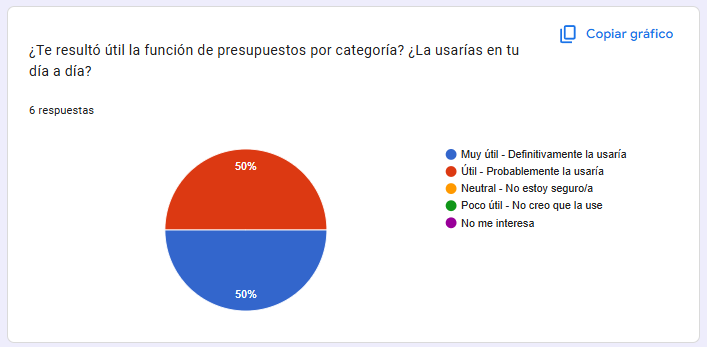
\includegraphics[width=0.8\textwidth]{images/imgAnexosPruebas/presupuestos_util.png}
		\caption{Utilidad percibida de los presupuestos por categoría.}
		\label{fig:pru-presupuestos}
	\end{figure}
	Respuestas sobre si los participantes usarían la función de presupuestos en su día a día.
}{}

\IfFileExists{images/imgAnexosPruebas/recibir_alertas.png}{
	\begin{figure}[H]
		\centering
		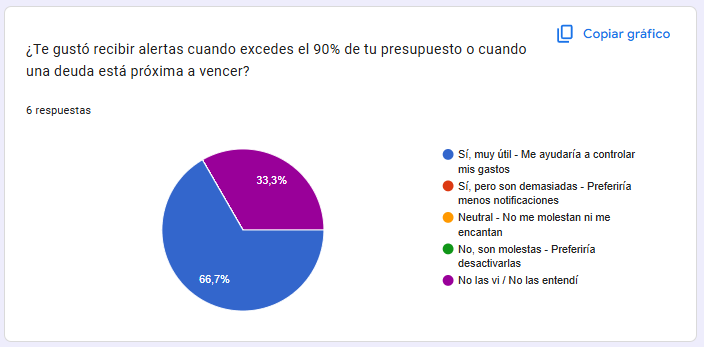
\includegraphics[width=0.8\textwidth]{images/imgAnexosPruebas/recibir_alertas.png}
		\caption{Percepción de las alertas automáticas del sistema.}
		\label{fig:pru-alertas}
	\end{figure}
	Valoración de las alertas por superación de presupuesto y vencimiento de deudas.
}{}

\IfFileExists{images/imgAnexosPruebas/graficasYestadisticas.png}{
	\begin{figure}[H]
		\centering
		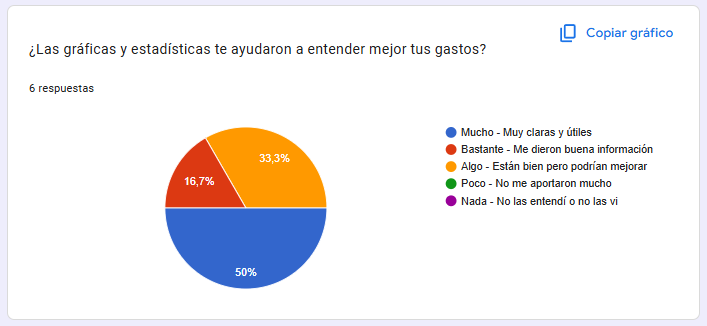
\includegraphics[width=0.8\textwidth]{images/imgAnexosPruebas/graficasYestadisticas.png}
		\caption{Utilidad de las gráficas y estadísticas de gastos.}
		\label{fig:pru-graficas}
	\end{figure}
	Grado en que las gráficas ayudaron a los participantes a entender sus gastos.
}{}

\IfFileExists{images/imgAnexosPruebas/nueva_funcionalidad.png}{
	\begin{figure}[H]
		\centering
		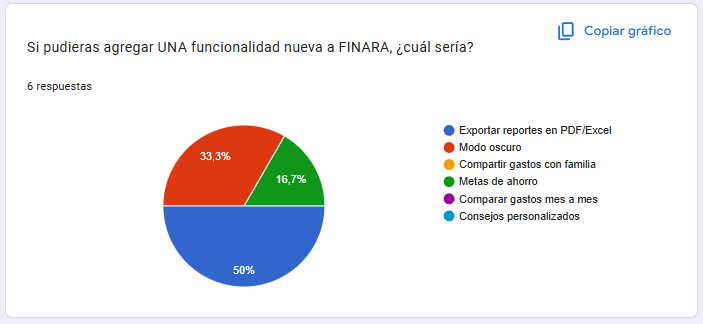
\includegraphics[width=0.8\textwidth]{images/imgAnexosPruebas/nueva_funcionalidad.png}
		\caption{Funcionalidad nueva más solicitada para versiones futuras.}
		\label{fig:pru-funcionalidad}
	\end{figure}
	Funcionalidad que los participantes añadirían a FINARA en una versión futura.
}{}

\IfFileExists{images/imgAnexosPruebas/registrar_gasto.png}{
	\begin{figure}[H]
		\centering
		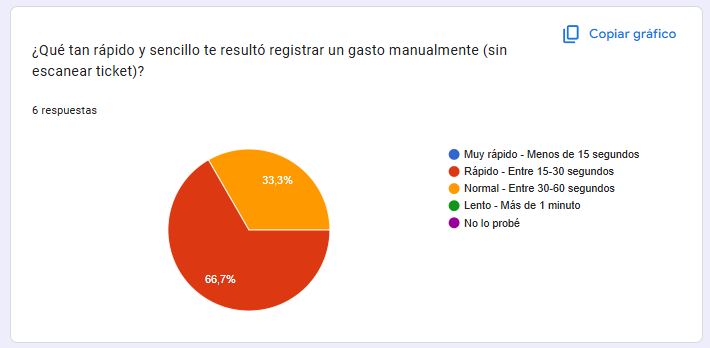
\includegraphics[width=0.8\textwidth]{images/imgAnexosPruebas/registrar_gasto.png}
		\caption{Rapidez para registrar un gasto manualmente.}
		\label{fig:pru-gasto}
	\end{figure}
	Tiempo percibido para completar el registro de un gasto sin escanear ticket.
}{}

\IfFileExists{images/imgAnexosPruebas/seccion_deudas.png}{
	\begin{figure}[H]
		\centering
		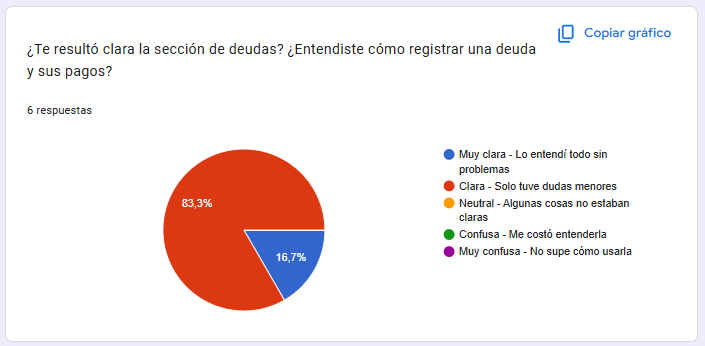
\includegraphics[width=0.8\textwidth]{images/imgAnexosPruebas/seccion_deudas.png}
		\caption{Claridad de la sección de deudas.}
		\label{fig:pru-deudas}
	\end{figure}
	Comprensión de los participantes sobre cómo registrar una deuda y sus pagos.
}{}

\IfFileExists{images/imgAnexosPruebas/recomiendas_finara.png}{
	\begin{figure}[H]
		\centering
		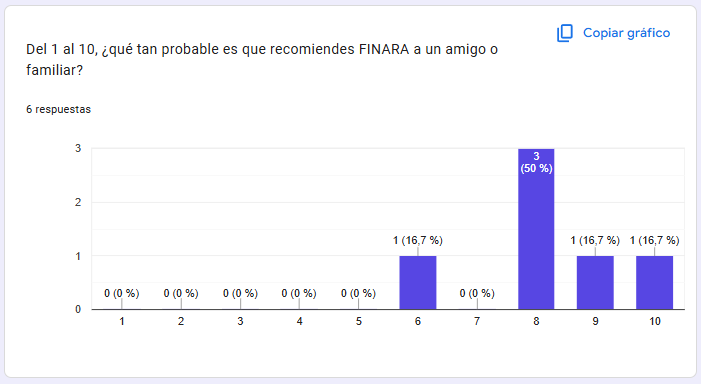
\includegraphics[width=0.8\textwidth]{images/imgAnexosPruebas/recomiendas_finara.png}
		\caption{Índice de recomendación (NPS) de FINARA.}
		\label{fig:pru-nps}
	\end{figure}
	Probabilidad (del 1 al 10) de que los participantes recomienden FINARA a un conocido.
}{}

\IfFileExists{images/imgAnexosPruebas/que_es_mejor.png}{
	\begin{figure}[H]
		\centering
		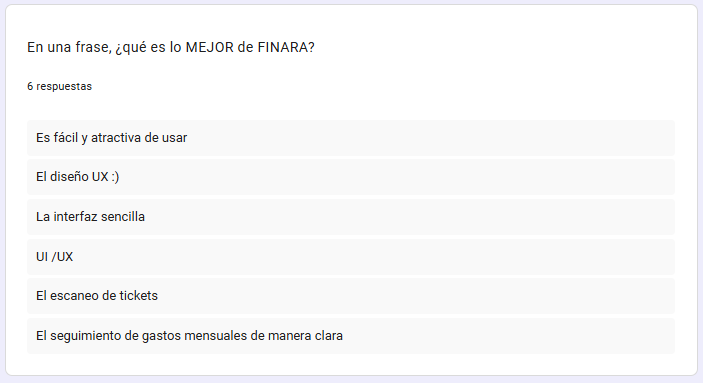
\includegraphics[width=0.8\textwidth]{images/imgAnexosPruebas/que_es_mejor.png}
		\caption{Lo mejor de FINARA según los usuarios.}
		\label{fig:pru-mejor}
	\end{figure}
	Respuestas abiertas sobre el aspecto más destacado de la aplicación.
}{}
